%%% Local Variables:
%%% mode: latex
%%% TeX-master: t
%%% End:

%%  commands definition and some other definitions about stuffs
\newcommand\here{lalala}
%\newcommand\x{x_i}
%\newcommand\y{y_i
\newcommand\dis{\displaystyle }


\subsection{}
\begin{frame}
  \frametitle{Linear Regression Example}
  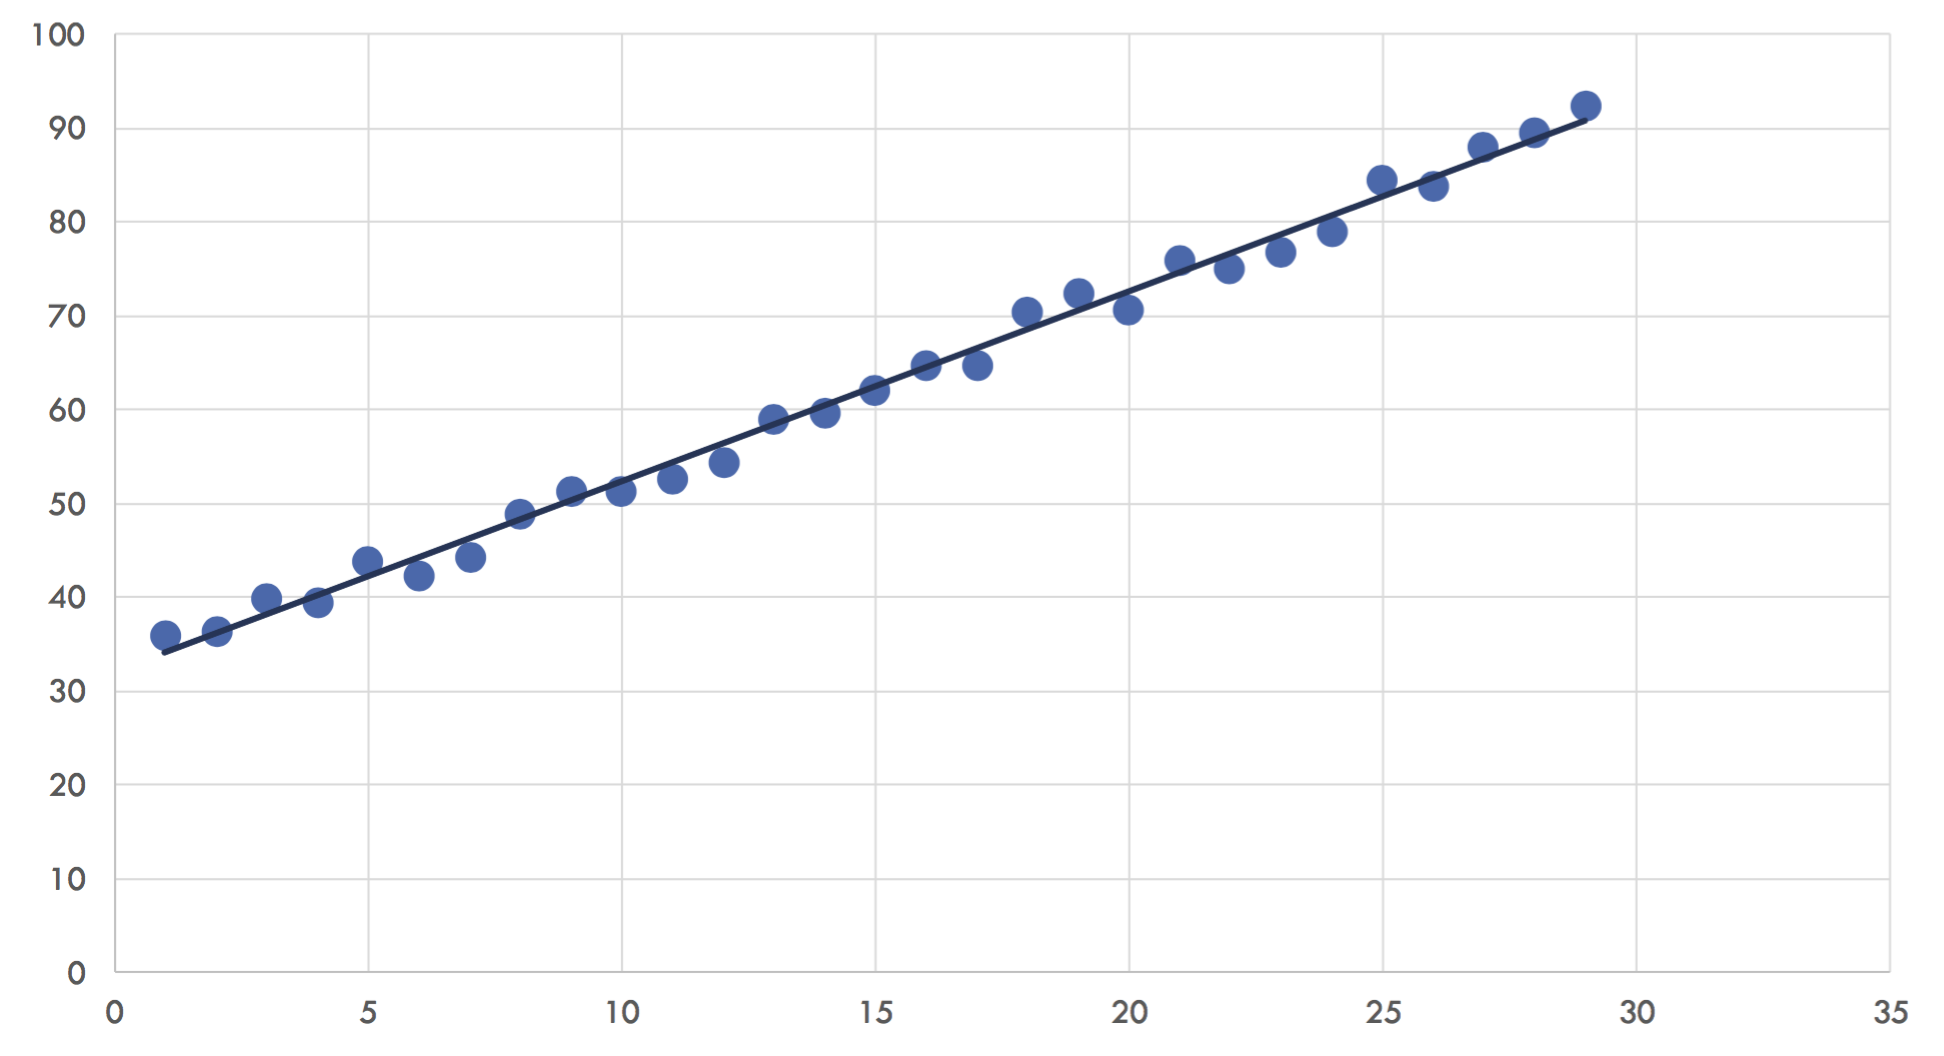
\includegraphics[scale=0.32]{pics/linear.png}

\end{frame}


\subsection{}
\begin{frame}
\frametitle{Ordinary Least Squares}

% 2 columns examples
\begin{columns}
  \begin{column}{0.6\textwidth}
    \begin{itemize}
    \item[] Input: points $(x_i, y_i)$
      \item[] Regression line: $y = mx + b$
\item[] Objective: $\displaystyle \min_{m, b} \sum_{i}(y_i - mx_i -b)^2$
    \end{itemize}
  \end{column}

  \begin{column}{0.5\textwidth}
    \begin{itemize}
    \item[] $(\vec{x_i}, y_i)$
    \item[] $y = \vec{w} \cdot \vec{x} + b$
    \item[] $\dis \min_{\vec{w}}\sum_{i}(y_i - \vec{w} \cdot \vec{x_i} -b)^2$
    \end{itemize}

  \end{column}
\end{columns}

\begin{itemize}
\item Easily Solved: $\vec{w}^*(X^TX)-X^T\vec{y}$
\item But what if $\dim\vec{x} $ is large?
\item What about other similar regressions?
\end{itemize}

\end{frame}

\subsection{}
\begin{frame}
\frametitle{Convex Optimization Problems}


\begin{itemize}
\item OrdinaryLinearRegression: $\dis \min_{\vec{w}}\sum_i(y_i -
  \vec{w} \cdot \vec{x_i})^2$
\item General: $\dis \min_xf(x)$ where $f(x)$ is convex
\item Set $C$ is convex $\Longleftrightarrow \forall x, y\in C, 0\le t
  \le 1: tx +(1 - t)y \in C$
\item Function $f : \mathbb{R}^n \rightarrow \mathbb{R}$ is convex if
  $\dom f$ is convex and $\exists x, y \in \dom f, 0\le t \le 1:$

\end{itemize}

\vspace{-4mm}

{\small
$$f(tx + (1 - t)y) \le tf(x) + (1 - t)f(y)$$
}

\vspace{-4mm}

\begin{columns}
  \begin{column}{0.5\textwidth}

\begin{itemize}
\item Unconstrained.
\end{itemize}

  \end{column}

  \begin{column}{0.5\textwidth}
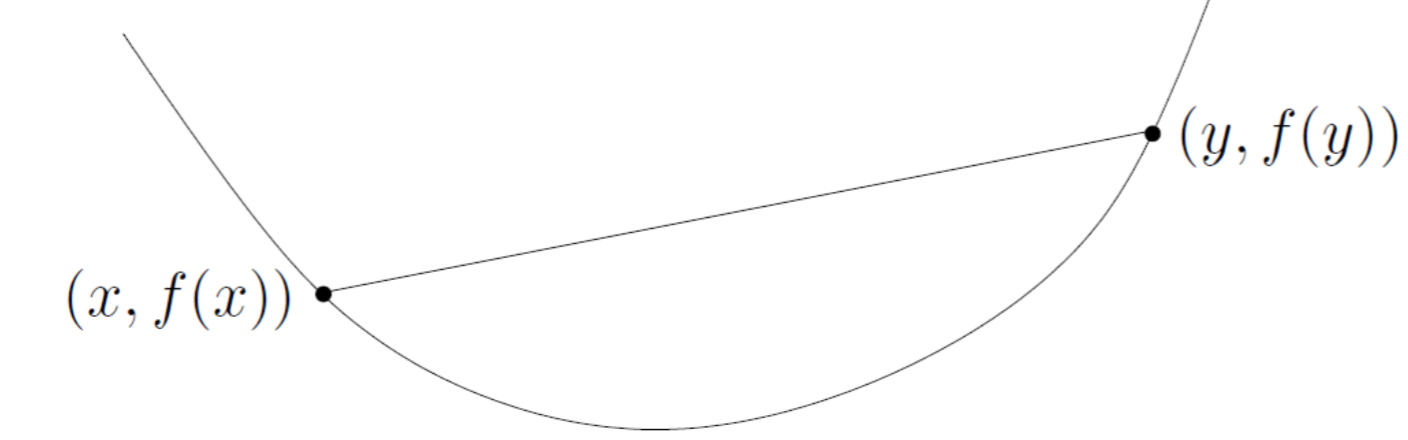
\includegraphics[scale=0.2]{pics/uncons.png}
  \end{column}
\end{columns}

\end{frame}

\subsection{}

\begin{frame}
  \frametitle{Outliers}
  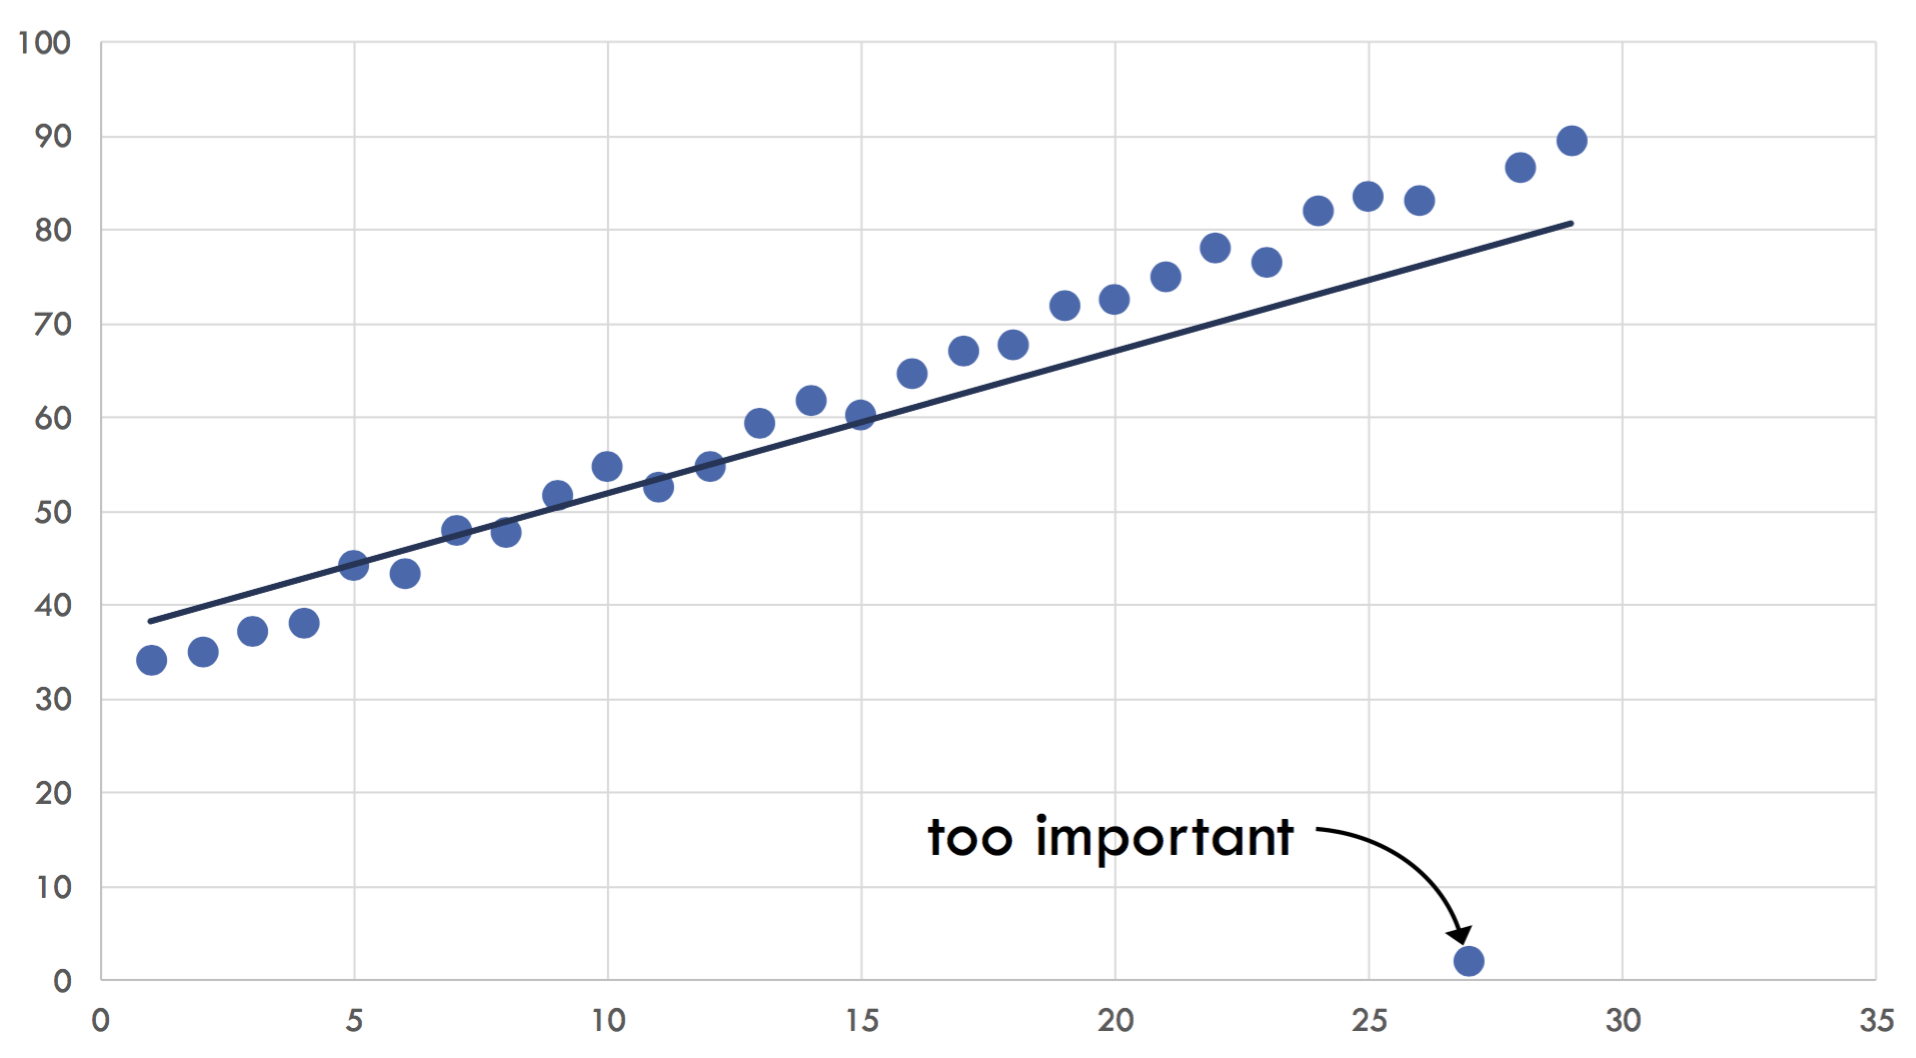
\includegraphics[scale=0.32]{pics/lpo.png}

\end{frame}

\subsection{}
\begin{frame}


  \frametitle{Outlier Penalty}

  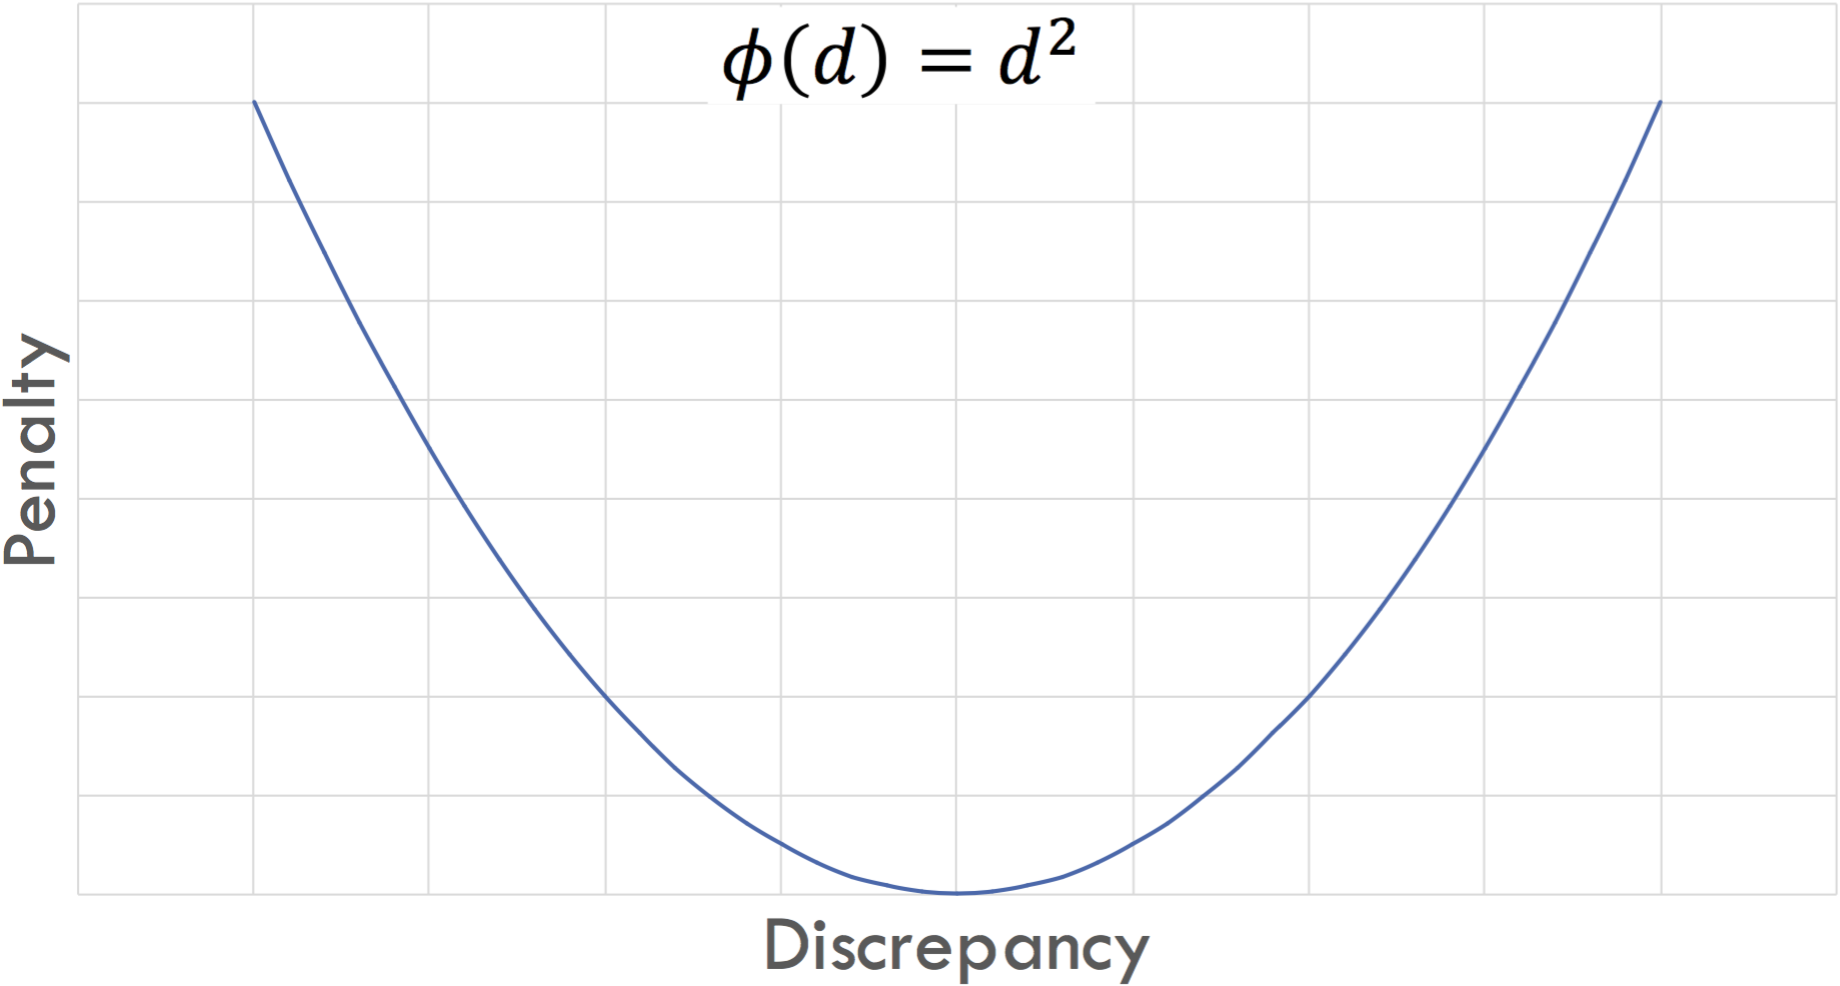
\includegraphics[scale=0.32]{pics/pen1.png}


\end{frame}

\begin{frame}
  \frametitle{Capped Penalty}
  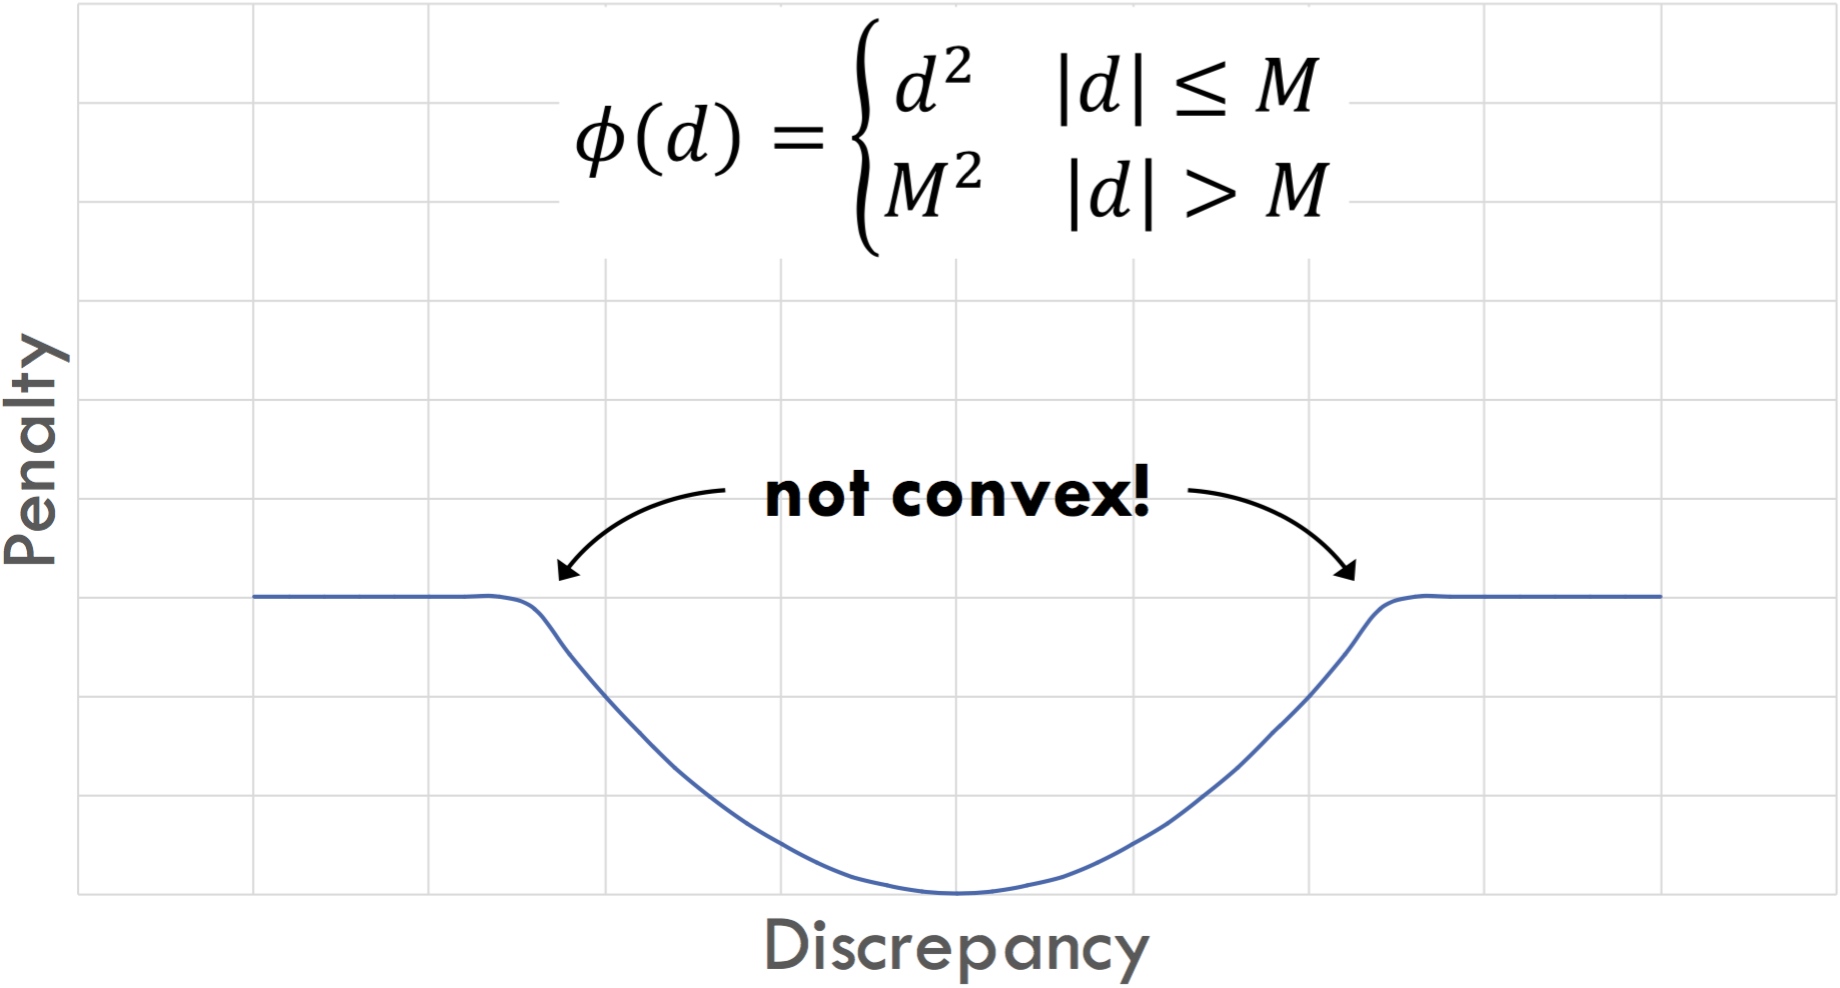
\includegraphics[scale=0.32]{pics/pen2.png}
\end{frame}

\begin{frame}
\frametitle{Huber Penalty Function}
  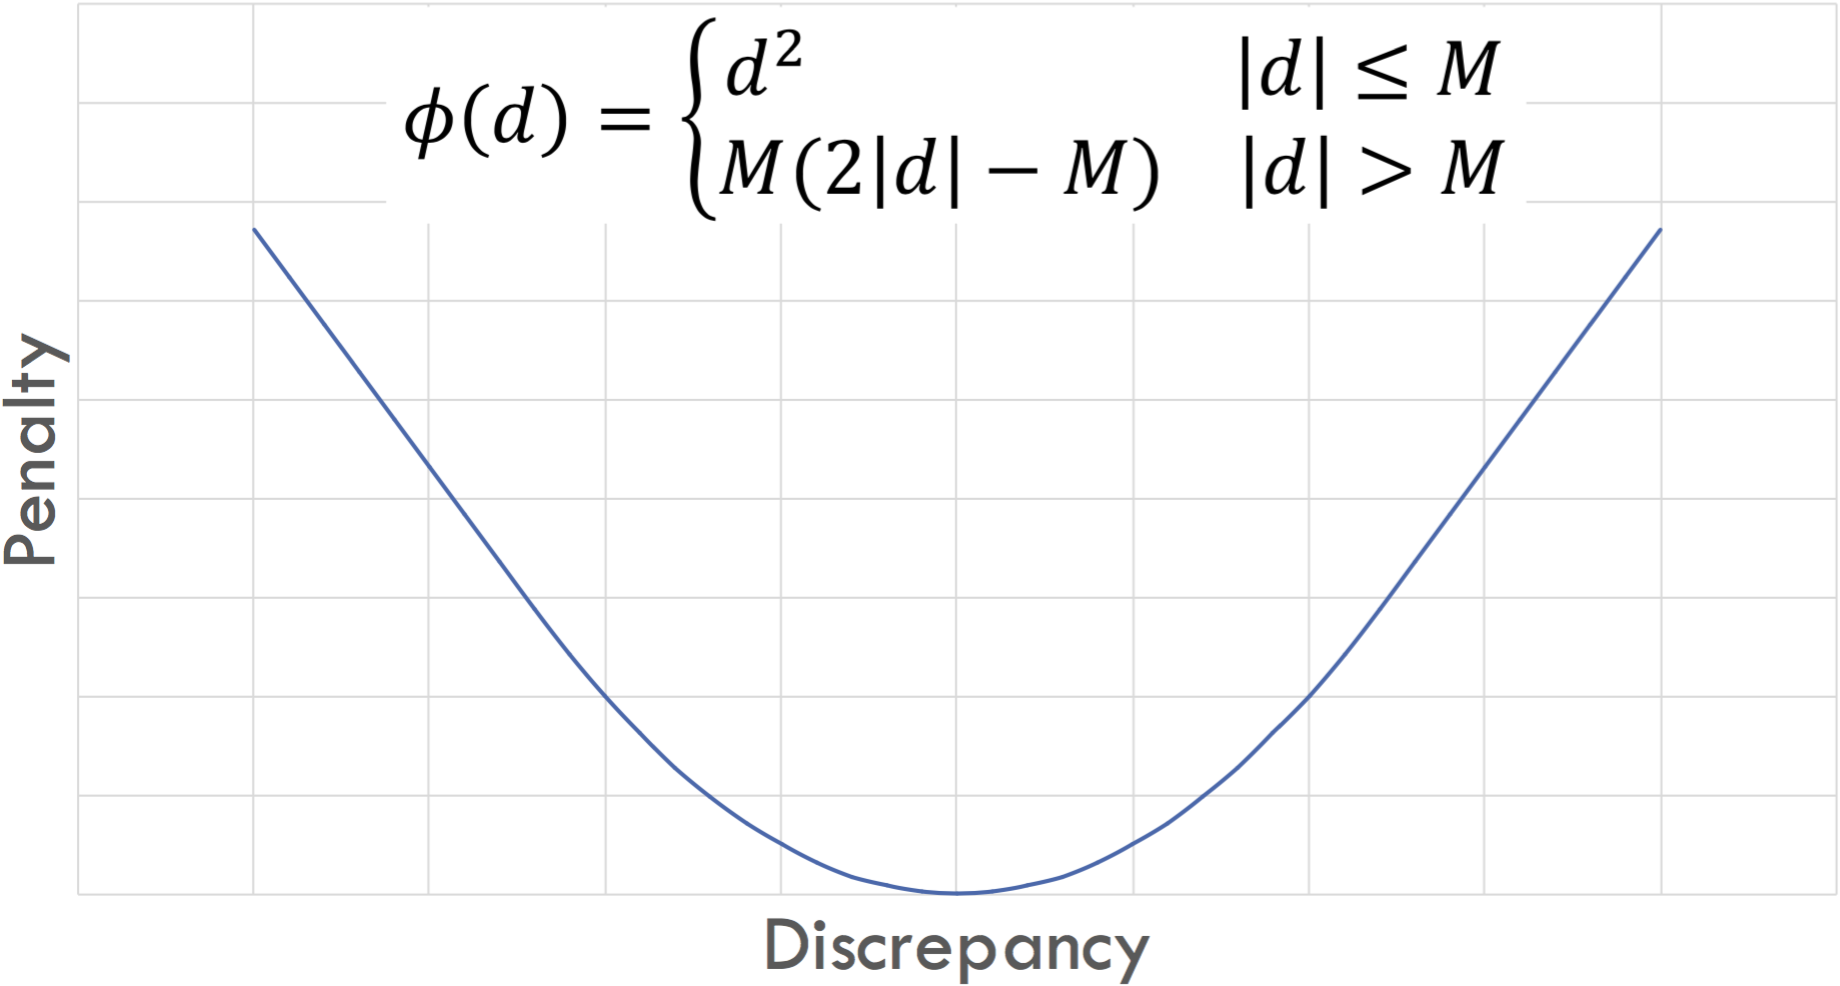
\includegraphics[scale=0.32]{pics/pen3.png}
\end{frame}
